%! Author = adrienkoumgangtegantchouang
%! Date = 09/07/24

\chapter{Modular Decomposition}\label{ch:modular-decomposition}


Modular decomposition is a fundamental concept in graph theory and combinatorial optimization that simplifies the analysis and processing of graphs.
By breaking down a graph into smaller, more manageable subgraphs known as modules, modular decomposition enables more efficient algorithms for various graph-related problems.
This chapter provides an overview of modular decomposition, including its definitions, properties, applications, and examples.


\section{Definition of graph}\label{sec:definition-of-graph}

A graph is a mathematical structure used to model pairwise relations between objects. \cite{GT1,GT2}

\begin{mydef}
    A graph $G$ is defined as an ordered pair $G = (V, E)$, where
    \begin{itemize}
        \item $V$ is a finite set of vertices (or nodes).
        \item $E$ is a set of edges (or arcs), where each edge is a pair of vertices.
    \end{itemize}
\end{mydef}

Graphs can be broadly categorized into two types based on the nature of their edges: undirected graphs and directed graphs.

\subsection*{Undirected Graph}\label{subsec:undirected-graph}

An undirected graph is a type of graph in which the edges have no orientation.
The edges simply connect two vertices and do not have a direction associated with them.

An undirected graph is a graph $G = (V, E)$ where $E \subseteq P_2(V)$, i.e., $E$ is a set of subsets of nodes of cardinality 2.
Therefore, each edge $\{u, v\}$ is an unordered pair of vertices.

In undirected graphs, the edge $\{u, v\}$ is identical to the edge $\{v, u\}$, implying that the connection is bidirectional.

\begin{myex}[An undirected graph~\cite{mdwikipedia}]
    An undirected graph $G$ with vertices $V = \{v1, v2, v3, v4, v5, v6, v7, v8, v9, v10, v11\}$ and edges \\
    $E= \{\{v1, v2\}, \{v1, v3\}, \{v1, v4\}\}$
    $\cup \; \{\{v2, v4\}, \{v2, v5\}, \{v2, v6\}, \{v2, v7\}\}$ \\
    $\cup \; \{\{v3, v4\}, \{v3, v5\}, \{v3, v6\}, \{v3, v7\}\}$
    $\cup \; \{\{v4, v5\}, \{v4, v6\}, \{v4, v7\}\}$
    $\cup \; \{\{v5, v6\}, \{v5, v7\}\}$
    $\cup \; \{\{v6, v8\}, \{v6, v9\}, \{v6, v10\}, \{v6, v11\}\}$
    $\cup \; \{\{v7, v8\}, \{v7, v9\}, \{v7, v10\}, \{v7, v11\}\}$
    $\cup \; \{\{v8, v9\}, \{v8, v10\}, \{v8, v11\}\}$
    $\cup \; \{\{v9, v10\}, \{v9, v11\}\}$

    \begin{figure}[!h]
        \centering
        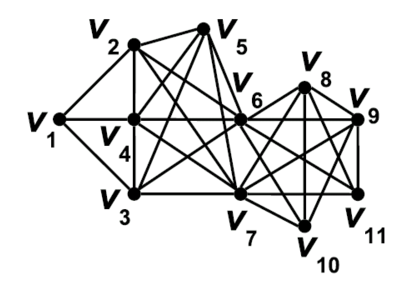
\includegraphics[width=0.40\textwidth]{images/graphs/undirected_graph_wikipedia}
        \caption{Example of Undirected Graph}
        \label{fig:example-undirected-graph}
    \end{figure}
\end{myex}

Undirected graphs are commonly used in scenarios where the relationships are mutual, such as social networks where friendships are bidirectional.

\subsection*{Directed Graph}\label{subsec:directed-graph}

A directed graph, or digraph, is a type of graph in which the edges have a direction, indicating a one-way relationship between the vertices.

A directed graph is a graph $G = (V, E)$ where $E \subseteq V \times V$, i.e., $E$ is a binary relation on $V$.
Therefore, each edge $(v, w)$ is an ordered pair of vertices.

In directed graphs, the edge $(u, v)$ is not identical to the edge $(v, u)$, implying that the connection is unidirectional.

\begin{myex}[A directed graph]
    A directed graph $G$ with vertices $V = \{1, 2, 3, 4, 5, 6, 7, 8\}$ and edges \\
    $E = \{(1, 2), (1, 3)\}$
    $\cup \; \{(2, 3)\}$
    $\cup \; \{(4 , 1), (4, 2), (4, 3), (4, 6)\}$
    $\cup \; \{(5 , 1), (5, 2), (5, 3), (5, 6)\}$
    $\cup \; \{(6, 4), (6, 5), (6, 7), (6, 8)\}$
    $\cup \; \{(7, 8)\}$
    $\cup \; \{(8, 7)\}$

    \begin{figure}[!h]
        \centering
        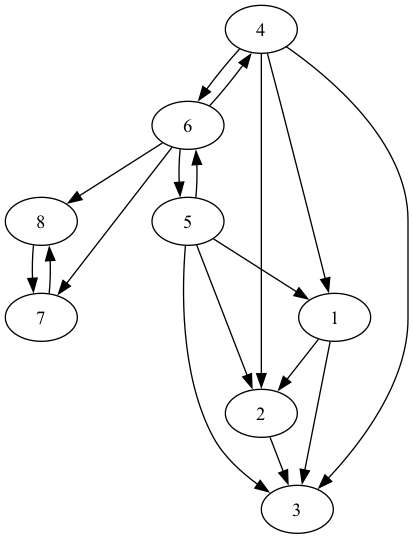
\includegraphics[width=0.40\textwidth]{images/graphs/digraph_ex1_without_label}
        \caption{Example of Directed Graph}
        \label{fig:example-directed-graph}
    \end{figure}
\end{myex}

Directed graphs are used where relationships have a direction, such as web page links (where one page links to another) or task scheduling (where one task must precede another).


\section{Definition of Modular Decomposition}\label{sec:definition-of-modular-decomposition}

\subsection*{Module}\label{subsec:module}

Modular decomposition involves partitioning the vertex set $V$ into subsets, or modules, that have specific properties relative to the rest of the graph.

A \textbf{module}~\cite{mdwikipedia} of a graph is a generalization of a connected component~\cite{componentwikipedia}.
In graph theory, a \textbf{component} of an undirected graph is a connected subgraph that is not part of any larger connected subgraph.
The components of any graph partition its vertices into disjoint sets, and are the induced subgraphs of those sets.
A graph that is itself connected has exactly one component, consisting of the whole graph.
Components are sometimes called \textbf{connected components}.

\begin{figure}[!h]
    \centering
    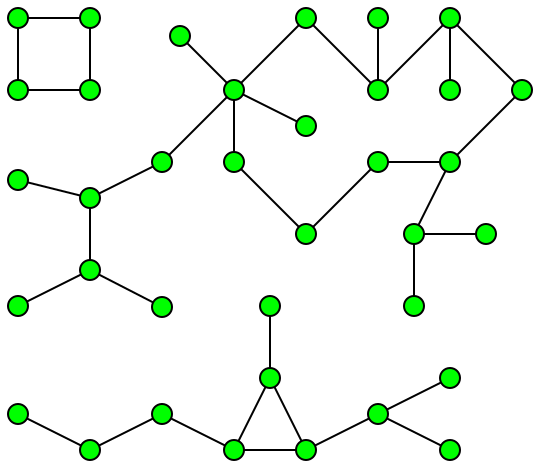
\includegraphics[width=0.40\textwidth]{images/graphs/Pseudoforest}
    \caption{Example of Modules (A graph with three components) \cite{componentwikipedia}}
    \label{fig:example-modules}
\end{figure}

A connected component has the property that it is a set $M$ of vertices such that every member of $M$ is a non-neighbor of every not vertex in $M$.
(It is a union of connected components if and only if it has this property.)
More generally, $M$ is a module if, for each vertex $m \notin M$, either every member of $M$ is a non-neighbor of $m$ or every member of $M$ is a neighbor of $m$.

Equivalently, $M$ is a module if all members of $M$ have the same set of neighbors among vertices not in $M$.

Another definition of components involves the equivalence classes of an equivalence relation defined on the graph's vertices.
In an undirected graph, a vertex $v$ is reachable from a vertex $u$, if there is a path from $u$ to $v$, or equivalently a walk (a path allowing repeated vertices and edges).
Reachability is an equivalence relation, since:
\begin{itemize}
    \item It is \textbf{reflexive}: There is a trivial path of length zero from any vertex to itself.
    \item It is \textbf{symmetric}: If there is a path from $u$ to $v$, the same edges in the reserve order from a path from $v$ to $u$.
    \item It is \textbf{transitive}: If there is a path from $u$ to $v$ and a path from $v$ to $w$, the two paths may be concatenated together to form a walk from $u$ to $w$.
\end{itemize}

\begin{mydef}
(Module)
    A module $M \subseteq V$ of a graph $G$ is a subset of vertices such that every vertex in $M$ has the same set of neighbors outside $M$.
    Formally, for any $u, v \in M$ and any $w \in V - M$, $w$ is adjacent to $u$ if and only if $w$ is adjacent to $v$.
\end{mydef}

This definition ensures that within a module, the vertices are indistinguishable based on their connections to the rest of the graph.
Modules can vary in size and structure, from single vertices to large subgraphs encompassing a significant portion of the original graph.

Contrary to the connected components, the modules of a graph are the same as the modules of its complement, and modules can be nested: one module can be a proper subset of another.
Note that the set $V$ of vertices of a graph is a module, as are its one-element subsets and the empty set; these are called the \textbf{trivial modules}.
A graph may or may not have other modules.
A graph is called \textbf{prime} if all of its modules are trivial.

\begin{mydef}[Prime module]
    A prime module is a module where the subgraph induced by the vertices of the module does not admit any non-trivial decomposition into smaller modules.
\end{mydef}

In the mathematical field of graph theory, the complement~\cite{complementgraphwikipedia} or inverse of a graph $G$ is a graph $H$ on the same vertices such that two distinct vertices of $H$ are adjacent if and only if they are not adjacent in $G$.
That is, to generate the complement of a graph, one fills in all the missing edges required to form a complete graph, and removes all the edges that were previously there.
The complement is not the set complement of the graph; only the edges are complemented.

\begin{figure}[!h]
    \centering
    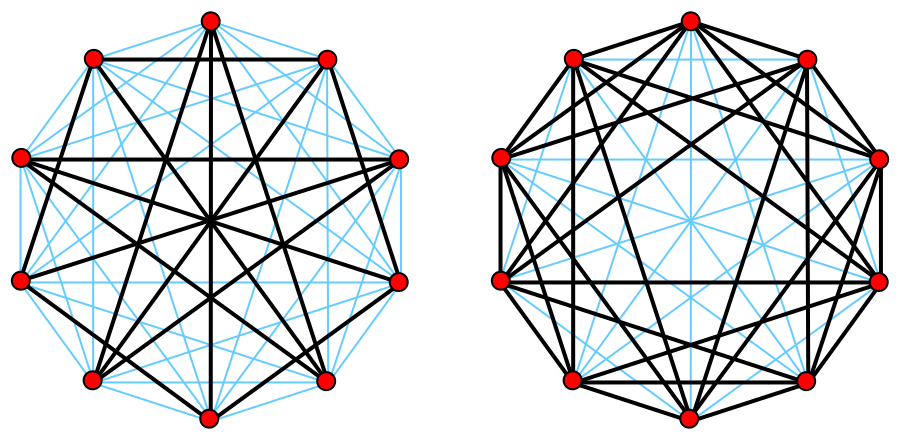
\includegraphics[width=0.40\textwidth]{images/graphs/Petersen_graph_complement}
    \caption{The Petersen graph (on the left) and its complement graph (on the right) \cite{complementgraphwikipedia}}
    \label{fig:the}
\end{figure}


\subsection*{Modular Partition}\label{subsec:modular-partition}

In graph theory, partitioning a graph into meaningful substructures is a common strategy for simplifying complex problems.
A modular partition specifically refers to dividing the vertices of a graph into disjoint subsets, known as modules, where each subset satisfies certain uniformity conditions relative to the rest of the graph.
This concept is crucial for understanding the deeper hierarchical structure of graphs and forms the foundation for various graph decomposition techniques.

\begin{mydef}
    A modular partition of a graph $G = (V, E)$ is a partition of the vertex set $V$ into disjoint subsets $M_1$, $M_2$, \ldots, $M_k$ such that each subset $M_i$ (for $i = 1, 2, \ldots, k$) is a module.
\end{mydef}

\subsubsection*{Properties of Modular Partitions}

Modular partitions possess several important properties that make them useful for graph analysis:

\begin{enumerate}
    \item \textbf{Uniform Neighborhood:} Within a module, all vertices share the same neighbors outside the module.
    This property allows for simplification of the graph by treating the entire module as a single unit when considering its external connections.
    \item \textbf{Independence from Internal Structure:} The internal structure of a module does not affect its status as a module.
    This means that the relationships between vertices within a module are irrelevant to the modular partitioning, focusing solely on external connections.
    \item \textbf{Hierarchical Organization:} Modular partitions naturally lead to a hierarchical organization of the graph.
    By recursively partitioning modules into smaller modules, one can build a modular decomposition tree that captures the multi-level structure of the graph.
\end{enumerate}

To illustrate the concept of modular partitions, consider the following examples:

\begin{myex}[Simple Undirected Graph]
    Consider an undirected graph $G$ from Figure~\ref{fig:example-undirected-graph}.

    In this graph, the sets $\{v2, v3, v4\}$ and $\{v6, v7\}$ each form modules.
    The non trivial modules are: $\{v2, v3\}, \{v2, v3, v4\}, \{v6, v7\}, \{v10, v11\}, \{v8, v9, v10, v11\}$.

    \begin{figure}[!h]
        \centering
        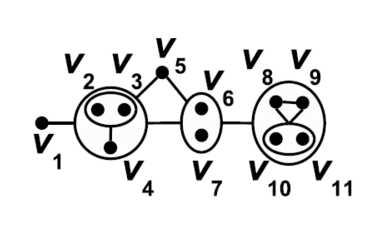
\includegraphics[width=0.40\textwidth]{images/graphs/undirected_graph_wikipedia_module}
        \caption{Example of Module for Simple Undirected Graph}
        \label{fig:example-undirected-graph-module}
    \end{figure}

    Possible modular partition are:
    \begin{itemize}
        \item $\{\{v1\}, \{v2, v3, v4\}, \{v5\}, \{v6, v7\}, \{v8, v9, v10, v11\}\}$
        \item $\{\{v1\}, \{v2, v3\}, \{v4\}, \{v5\}, \{v6, v7\}, \{v8\}, \{v9\}, \{v10, v11\}\}$
    \end{itemize}
    The last one is the maximal modular partition.
\end{myex}

\begin{myex}[Directed Graph]
    Consider a directed graph $G$ from Figure~\ref{fig:example-directed-graph}.

    In this graph, the sets $\{2, 3\}$, $\{4, 5\}$, and $\{6, 7, 8\}$ each form modules.
    Thus, a possible modular partition of $G$ is $\{\{1\}, \{2, 3\}, \{4, 5\}, \{6, 7, 8\}\}$.
\end{myex}

\subsection*{Maximal Modular Partition}\label{subsec:maximal-modular-partition}

The maximal modular partition of a graph is unique and consists of the largest possible prime modules.
Prime modules are those that cannot be further decomposed into smaller non-trivial modules.

\begin{mydef}
(Maximal modular partition)
    A maximal modular partition is a partition of a graph into modules, where the modules are maximal in the sense that they cannot be further partitioned into smaller modules.
\end{mydef}


\section{Application to 2-Structures}\label{sec:application-to-2-structures}

Modular decomposition extends naturally to 2-structures, which are complete directed graphs with arcs colored from a set of $k$ colors.
The additional complexity of orientation and coloring requires modified definitions and algorithms for modular decomposition.

A 2-structure is a generalization of a graph where edges (or arcs) between vertices are assigned different colors or types, capturing more complex relationships between vertices.
This concept is particularly useful in scenarios where the simple binary relationship (edge or no edge) in standard graphs is insufficient to model the nuances of the interactions between entitites.

\begin{mydef}
    A 2-structure $G$ is defined as a pair $G = (V, A)$, where
    \begin{itemize}
        \item $V$ is a finite set of vertices.
        \item $A$ is a set of arcs, where each arc is a triple $(u, v, c)$ consisting of an ordered pair of vertices $u$ and $v$, and a color or type $c$.
    \end{itemize}
\end{mydef}

In a 2-structure, the arc $(u, v, c)$ indicates a directed relationship from vertex $u$ to vertex $v$ with a specific color or type $c$.

Here are the properties of the 2-structures:

\begin{enumerate}
    \item \textbf{Directed and Colored Arcs:} Unlike standard graphs where edges are typically uncolored, 2-structures have arcs that are both directed and colored.
    This allows for a richer representation of relationships.
    \item \textbf{Complex Relationships:} The use of colors or types for arcs allows 2-structures to model complex relationships between vertices, where the nature of the relationship is significant.
    \item \textbf{Generalization:} 2-structures generalize both undirected and directed graphs.
    An undirected graph can be seen as a 2-structure where each edge is represented by two directed arcs of the same color (one in each direction).
    A directed graph is a 2-structure where arcs are colored uniformly.
\end{enumerate}

\begin{myex}[2-Structure]
    Consider a 2-structure $G$ with vertices $V = \{u, v, w, x\}$ and arcs $A = \{(u, v, 1), (u, w, 1), (v, w, 2), (w, x, 1)\}$, where the third element in each triple represents the color of the arc.

    \begin{figure}[!h]
        \centering
        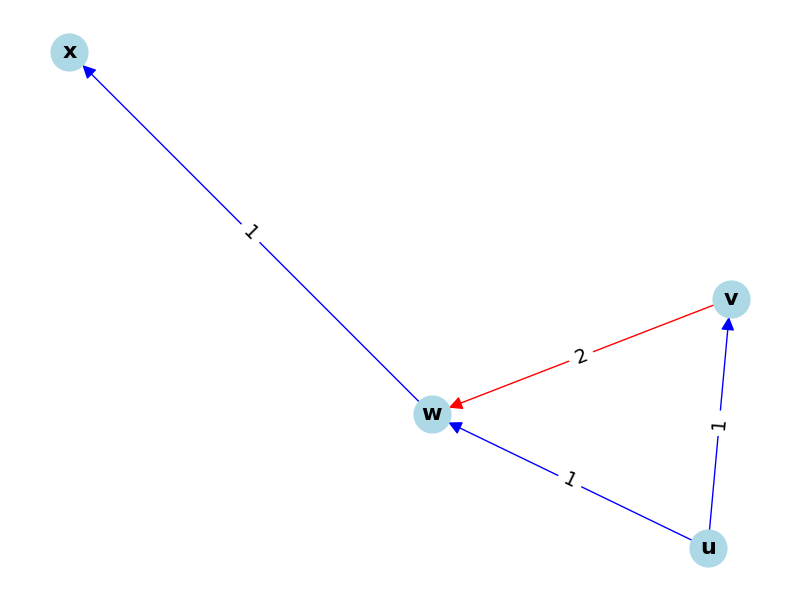
\includegraphics[width=0.40\textwidth]{images/graphs/2_structure_graph_example}
        \caption{Example of 2 Structure Graph}
        \label{fig:2-structure-graph-example-simple}
    \end{figure}

    In this 2-structure:
    \begin{itemize}
        \item The set of vertices $V$ is $\{u, v, w, x\}$
        \item The set of arcs $A$ includes:
        \begin{itemize}
            \item $(u, v, 1)$ indicating a type-1 arc from $u$ to $v$.
            \item $(u, w, 1)$ indicating a type-1 arc from $u$ to $w$.
            \item $(v, w, 2)$ indicating a type-2 arc from $v$ to $w$.
            \item $(w, x, 1)$ indicating a type-1 arc from $w$ to $x$.
        \end{itemize}
    \end{itemize}
\end{myex}

Another example of 2-structure from directed graph is Figure~\ref{fig:example-directed-graph}.


The definition of modules in 2-structures incorporates both the direction and color of arcs.

\begin{mydef}
    A module $M$ in a 2-structure $G$ is a subset of vertices such that for any $u, v \in M$ and any $w \in V - M$, the arcs $(w, u, c)$ and $(w, v, c)$ have the same color and direction, and the arcs $(u, w, c)$ and $(v, w, c)$ have the same color and direction.
\end{mydef}


\section{Examples of Modular Decomposition}\label{sec:examples-of-modular-decomposition}

To illustrate the concept of modular decomposition, consider the following examples.

% \subsection*{Example 1: Simple Undirected Graph}\label{subsec:example-1:-simple-undirected-graph}

\begin{myex}[Simple Undirected Graph]
    \label{ex:simple-undirected-graph}

Consider an undirected graph $G$ from Figure~\ref{fig:example-undirected-graph} and Figure~\ref{fig:example-undirected-graph-module}, the non-trivial modules of this graph are:

\begin{itemize}
    \item $\{v2, v3, v4\}$.
    \item $\{v6, v7\}$.
    \item $\{v8, v9, v10, v11\}$.
\end{itemize}

The maximal modular partition of $G$ is $\{\{v1\}, \{v2, v3\}, \{v4\}, \{v5\}, \{v6, v7\},$ \\ $\{v8\}, \{v9\}, \{v10, v11\}\}$.
\end{myex}

\begin{myex}[Directed Graph (2-structure)]
    Consider a directed graph $G$ from Figure~\ref{fig:example-directed-graph}.

    The non-trivial modules of this graph are $\{2, 3\}$, $\{4, 5\}$ and $\{7, 8\}$

    The maximal modular partition of $G$ is $\{\{1\}, \{2, 3\}, \{4, 5\}, \{6\}, \{7, 8\}\}$.
\end{myex}


\section{Modular Decomposition Tree}\label{sec:modular-decomposition-tree}

A modular decomposition tree is a tree structure that represents the hierarchical modular decomposition of a graph.

Structure of the Modular Decomposition Tree:
\begin{itemize}
    \item \textbf{Nodes:} Each node in the tree represents a module of the graph.
            \begin{itemize}
                \item \textbf{Leaf Nodes:} These correspond to individual vertices of the graph.
                \item \textbf{Internal Nodes:} These represent a module and are labeled with one of three types:
                        \begin{itemize}
                            \item \textbf{Parallel Node (P-node)}: Represents a module where the directed sub-modules form a set of disjoint independent sets (no edges between vertices within the module).
                            \item \textbf{Series Node (S-node)}: Represents a module where the directed sub-module form a clique (complete subgraph).
                            \item \textbf{Prime Node}: Represents a module where the module cannot be decomposed further into either parallel or series modules.
                        \end{itemize}
            \end{itemize}
    \item \textbf{Root:} The root node of the tree represents the entire graph.
\end{itemize}


\begin{Example}
    Consider the graph $G$ from Figure~\ref{fig:example-undirected-graph} with maximal modular partition \\ $\{\{v1\}, \{v2, v3, v4\}, \{v5\}, \{v6, v7\}, \{v8, v9\}, \{v10, v11\}\}$ (Figure~\ref{fig:example-undirected-graph-module}).
    The modular decomposition tree is constructed as follows:

    \begin{figure}[!h]
        \centering
        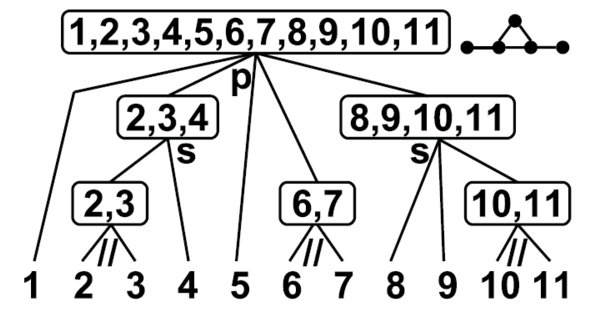
\includegraphics[width=0.40\textwidth]{images/graphs/undirected_graph_wikipedia_modular_decomposition}
        \caption{Example of Modular Decomposition Tree}
        \label{fig:example-undirected-graph-modular-decomposition-tree}
    \end{figure}
\end{Example}


\section{Applications of Modular Decomposition}\label{sec:applications-of-modular-decomposition}

Modular decomposition has numerous applications in various fields, including:

\subsection*{Bioinformatics}\label{subsec:bioinformatics}

In bioinformatics, modular decomposition is used to analyze and understand the structure of biological networks~\cite{MDPPIN}, such as protein-protein interaction networks and gene regulatory networks.
By decomposing these networks into modules, researchers can identify functional units and study their interactions.

\subsection*{Social Network Analysis}\label{subsec:social-network-analysis}

In social network analysis, modular decomposition helps identify communities or groups within a social network~\cite{NCCD}.
By understanding the modular structure, analysts can uncover patterns of interaction, influence, and information flow within the network.

\subsection*{Communication Networks}\label{subsec:communication-networks}

In communication networks, modular decomposition is used to optimize network design and routing~\cite{MANTP}.
By decomposing the network into modules, network engineers can develop efficient routing algorithms and improve the overall performance and reliability of the network.

% \section*{Conclusion}\label{sec:conclusion}

\hspace{4cm}

Modular decomposition is a powerful tool in graph theory that simplifies the analysis and processing of complex graphs.
By breaking down a graph into smaller modules, it enables more efficient algorithms and provides valuable insights into the structure and properties of the graph.
This chapter has provided a comprehensive overview of modular decomposition, including its definitions, properties, applications, and examples.
The subsequent chapters will delve into the algorithmic implementation of modular decomposition and its performance evaluation.

